\section{Assignment 1}

\subsection{Implement in MATLAB 3rd-, 5th-, 7th-order polynomials for $q_i>q_f$ and $q_i<q_f$ and for $t\in [t_i,t_f]$ and $t\in[0,\Delta T]$}

All polynomial trajectories can be expressed as:

\begin{align*}
q(t) &= a_7(t-t_i)^7 + a_6(t-t_i)^6 + a_5(t-t_i)^5 + a_4(t-t_i)^4 + a_3(t-t_i)^3 + a_2(t-t_i)^2 + a_1(t-t_i) + a_0\\
\dot q(t) &= 7a_7(t-t_i)^6 + 6a_6(t-t_i)^5 + 5a_5(t-t_i)^4 + 4a_4(t-t_i)^3 + 3a_3(t-t_i)^2 + 2a_2(t-t_i) + a_1\\
\ddot q(t) &= 42a_7(t-t_i)^5 + 30a_6(t-t_i)^4+20a_5(t-t_i)^3 + 12a_4(t-t_i)^2 + 6a_3(t-t_i) + 2a_2\\
\dddot q(t) &= 210a_7(t-t_i)^4 + 120a_6(t-t_i)^3+60a_5(t-t_i)^2 + 24a_4(t-t_i) + 6a_3\\
\ddddot q(t) &= 840a_7(t-t_i)^3 + 360a_6(t-t_i)^2+120a_5(t-t_i) + 24a_4
\end{align*}

For the 3rd-order polynomial $a_7=a_6=a_5=a_4=0$ while for the 5th-order polynomial $a_7=a_6=0$.

The problem of determining the $a_i$ coefficients of the polynomials is solved by setting up a system of equations using initial and final conditions on velocity (3rd-order), velocity and acceleration (5th-order), velocity, acceleration and jerk (7th-order).

\begin{figure}[H]
\centering
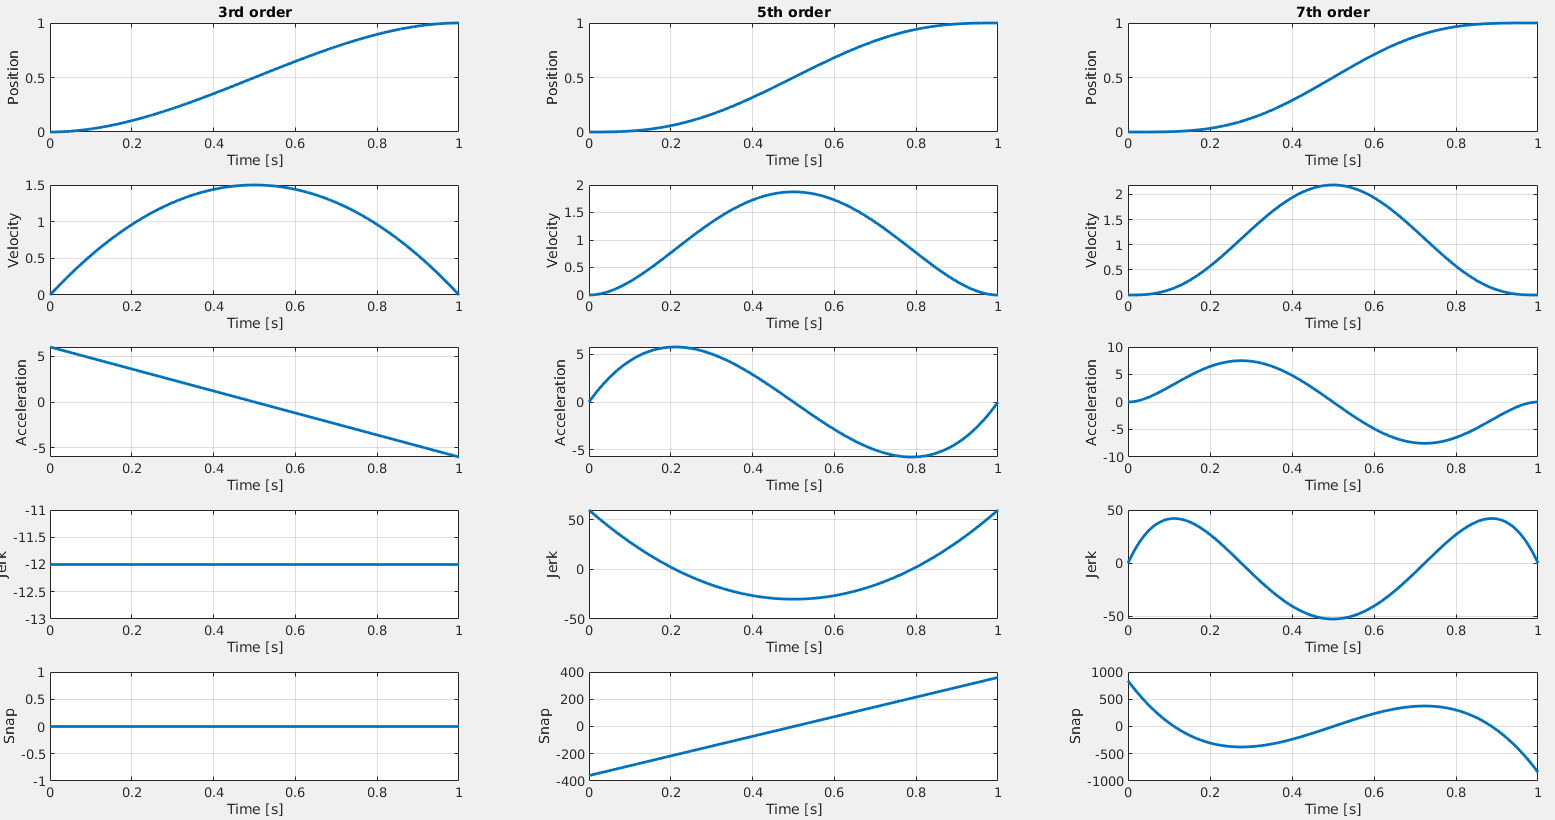
\includegraphics[keepaspectratio,width=\textwidth]{poly_1}
\caption{3rd-, 5th-, 7th-order polynomial trajectories with $q_i<q_f$ and $t\in[0,\Delta T]$, $q_i=0,q_f=1,\Delta T=1, v_i=v_f=a_i=a_f=j_i=j_f=0$.}
\label{fig:poly_1}
\end{figure}

\begin{figure}[H]
\centering
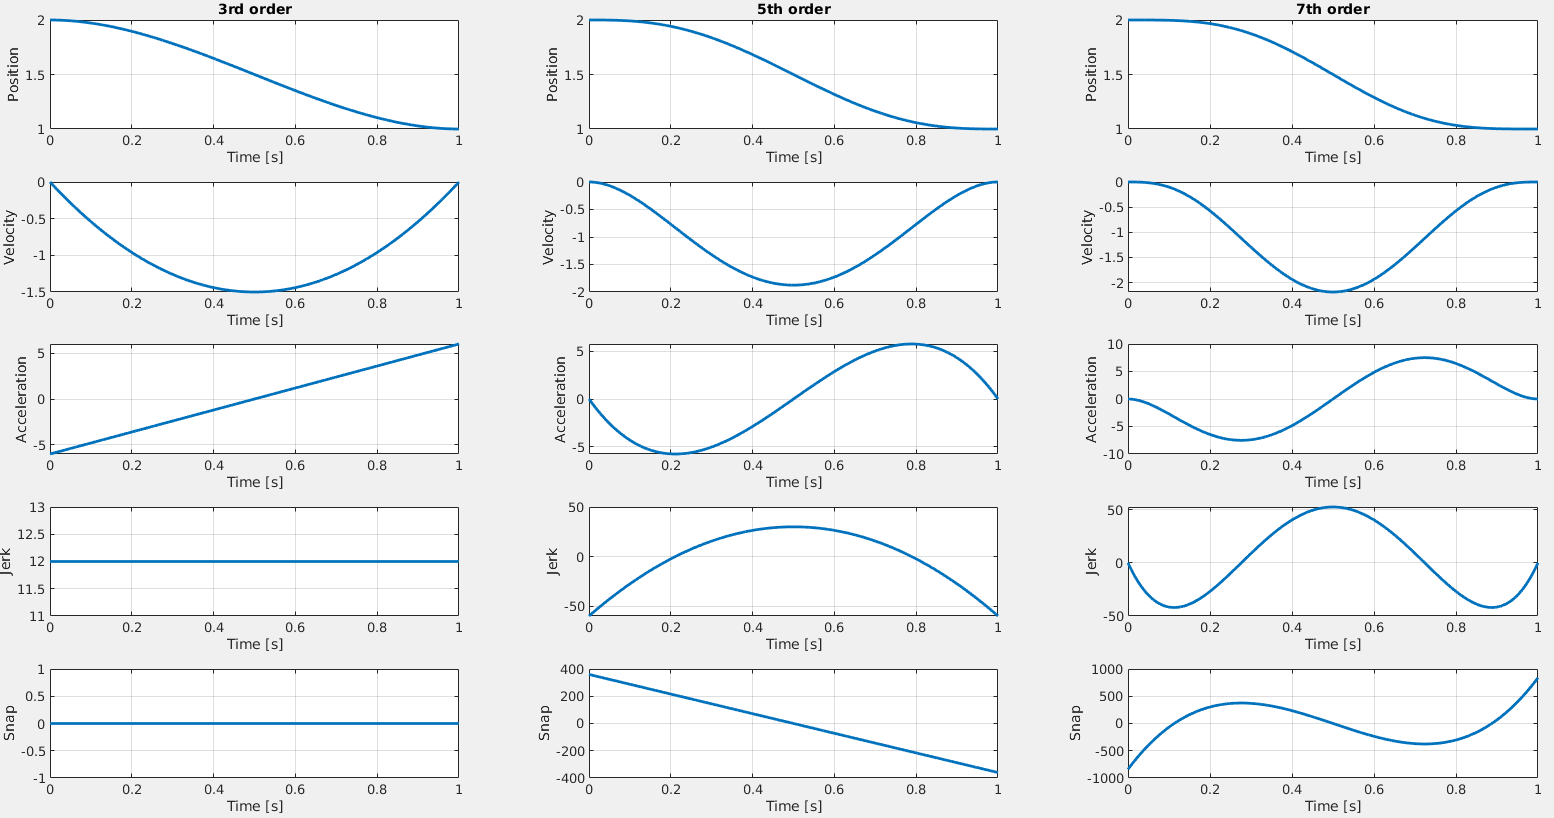
\includegraphics[keepaspectratio,width=\textwidth]{poly_2}
\caption{3rd-, 5th-, 7th-order polynomial trajectories with $q_i>q_f$ and $t\in[0,\Delta T]$, $q_i=2,q_f=1,\Delta T=1, v_i=v_f=a_i=a_f=j_i=j_f=0$.}
\label{fig:poly_2}
\end{figure}

\begin{figure}[H]
\centering
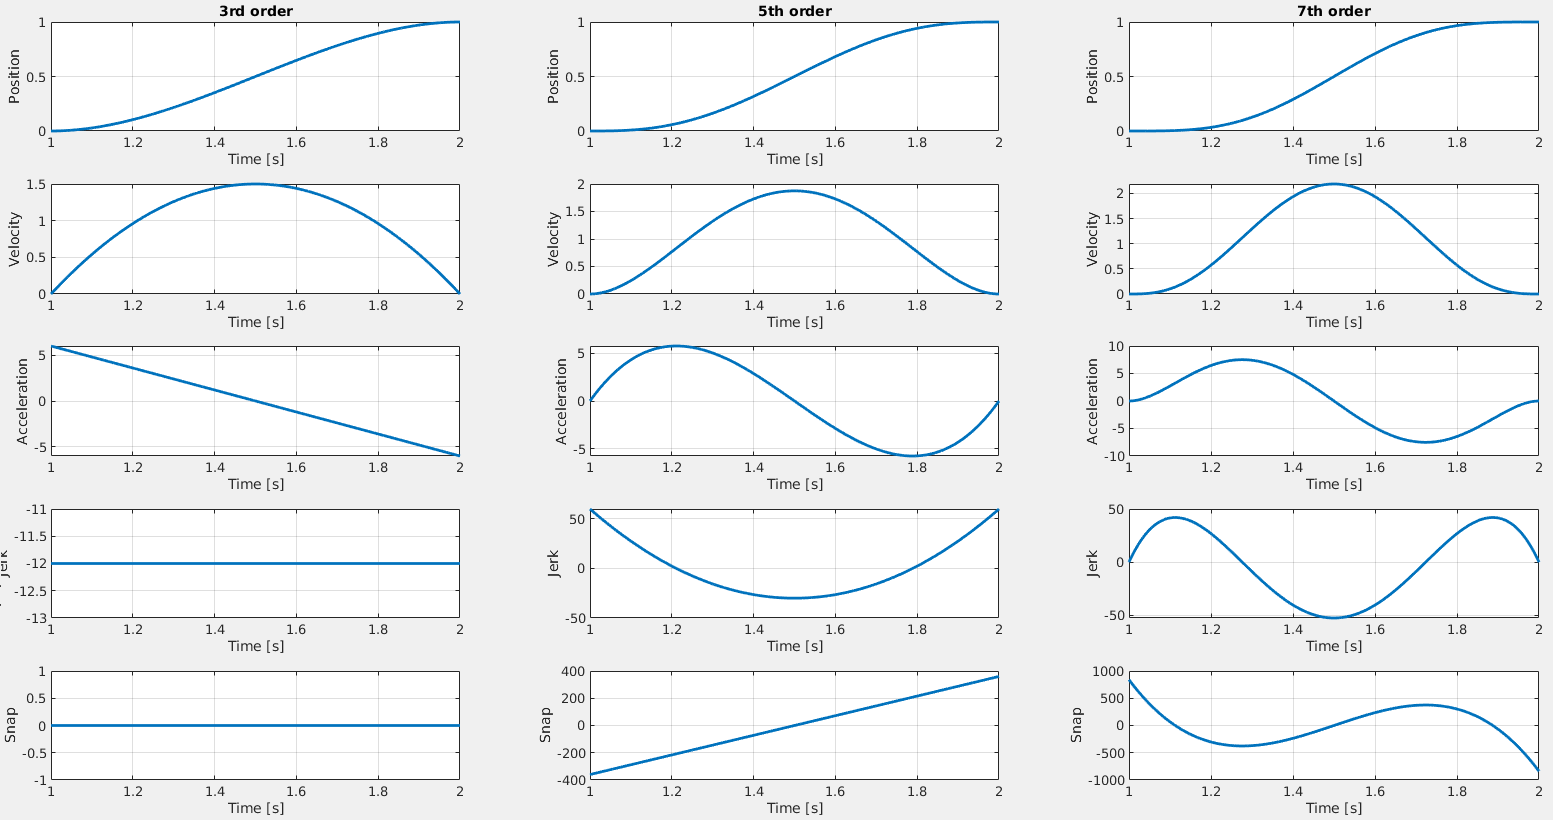
\includegraphics[keepaspectratio,width=\textwidth]{poly_3}
\caption{3rd-, 5th-, 7th-order polynomial trajectories with $q_i<q_f$ and $t\in[t_i,t_f]$, $q_i=0,q_f=1,t_i=1,t_f=2, v_i=v_f=a_i=a_f=j_i=j_f=0$.}
\label{fig:poly_3}
\end{figure}

\begin{figure}[H]
\centering
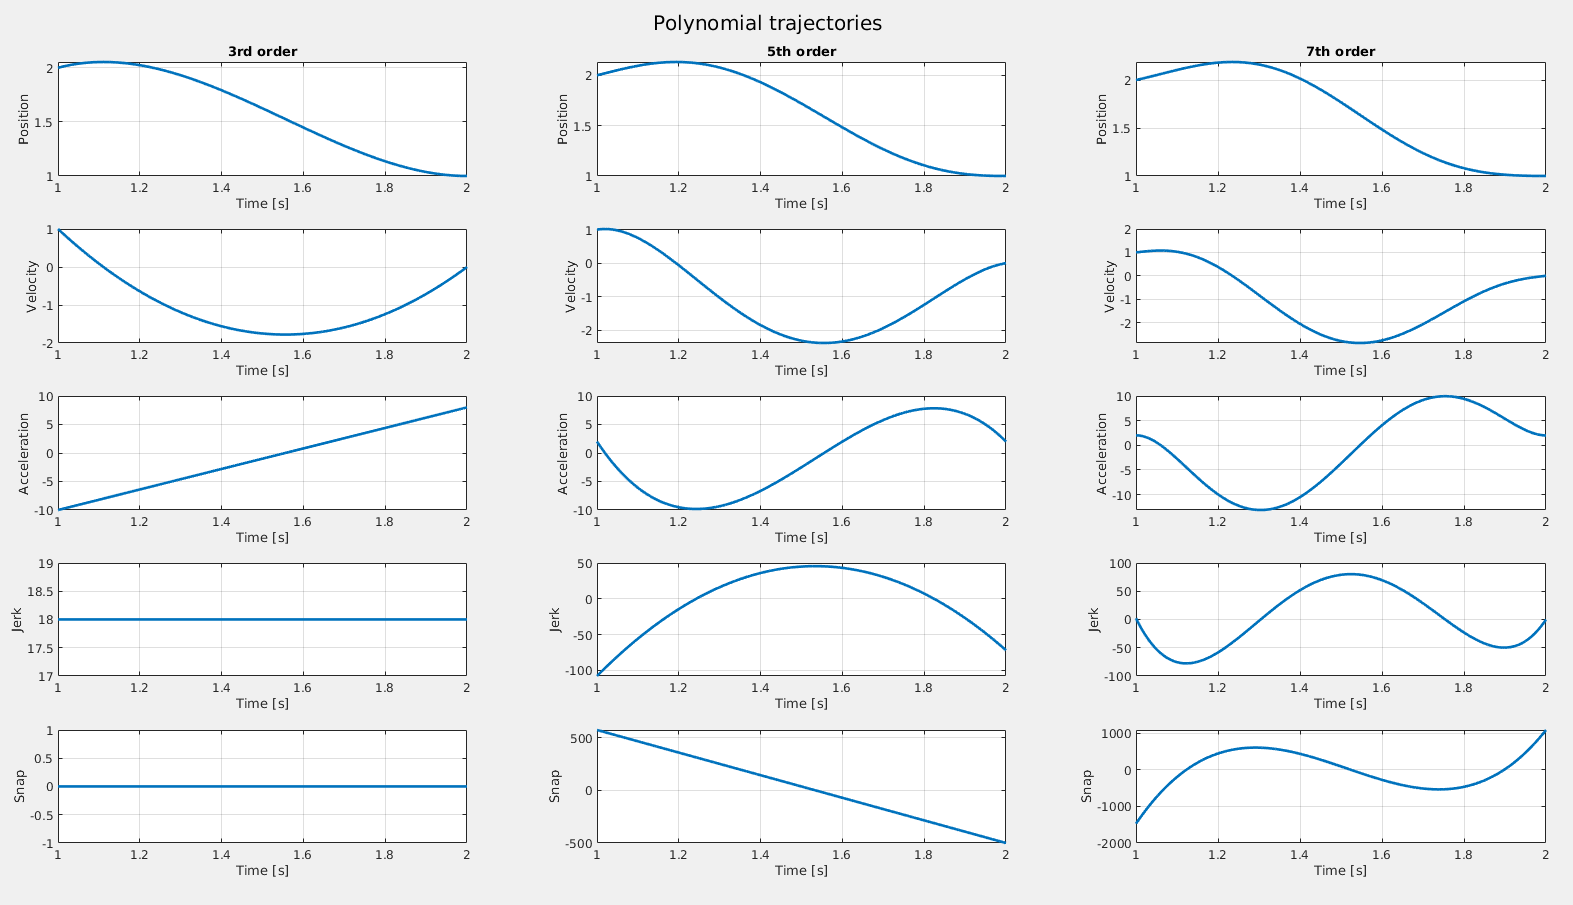
\includegraphics[keepaspectratio,width=\textwidth]{poly_4}
\caption{3rd-, 5th-, 7th-order polynomial trajectories with $q_i>q_f$ and $t\in[t_i,t_f]$, $q_i=2,q_f=1,t_i=1,t_f=2, v_i=1,v_f=0,a_i=2,a_f=2,j_i=2,j_f=0$.}
\label{fig:poly_4}
\end{figure}